\begin{appendix}

    \chapter{Abbildungen}

        \begin{figure}[ht]
            \centering
            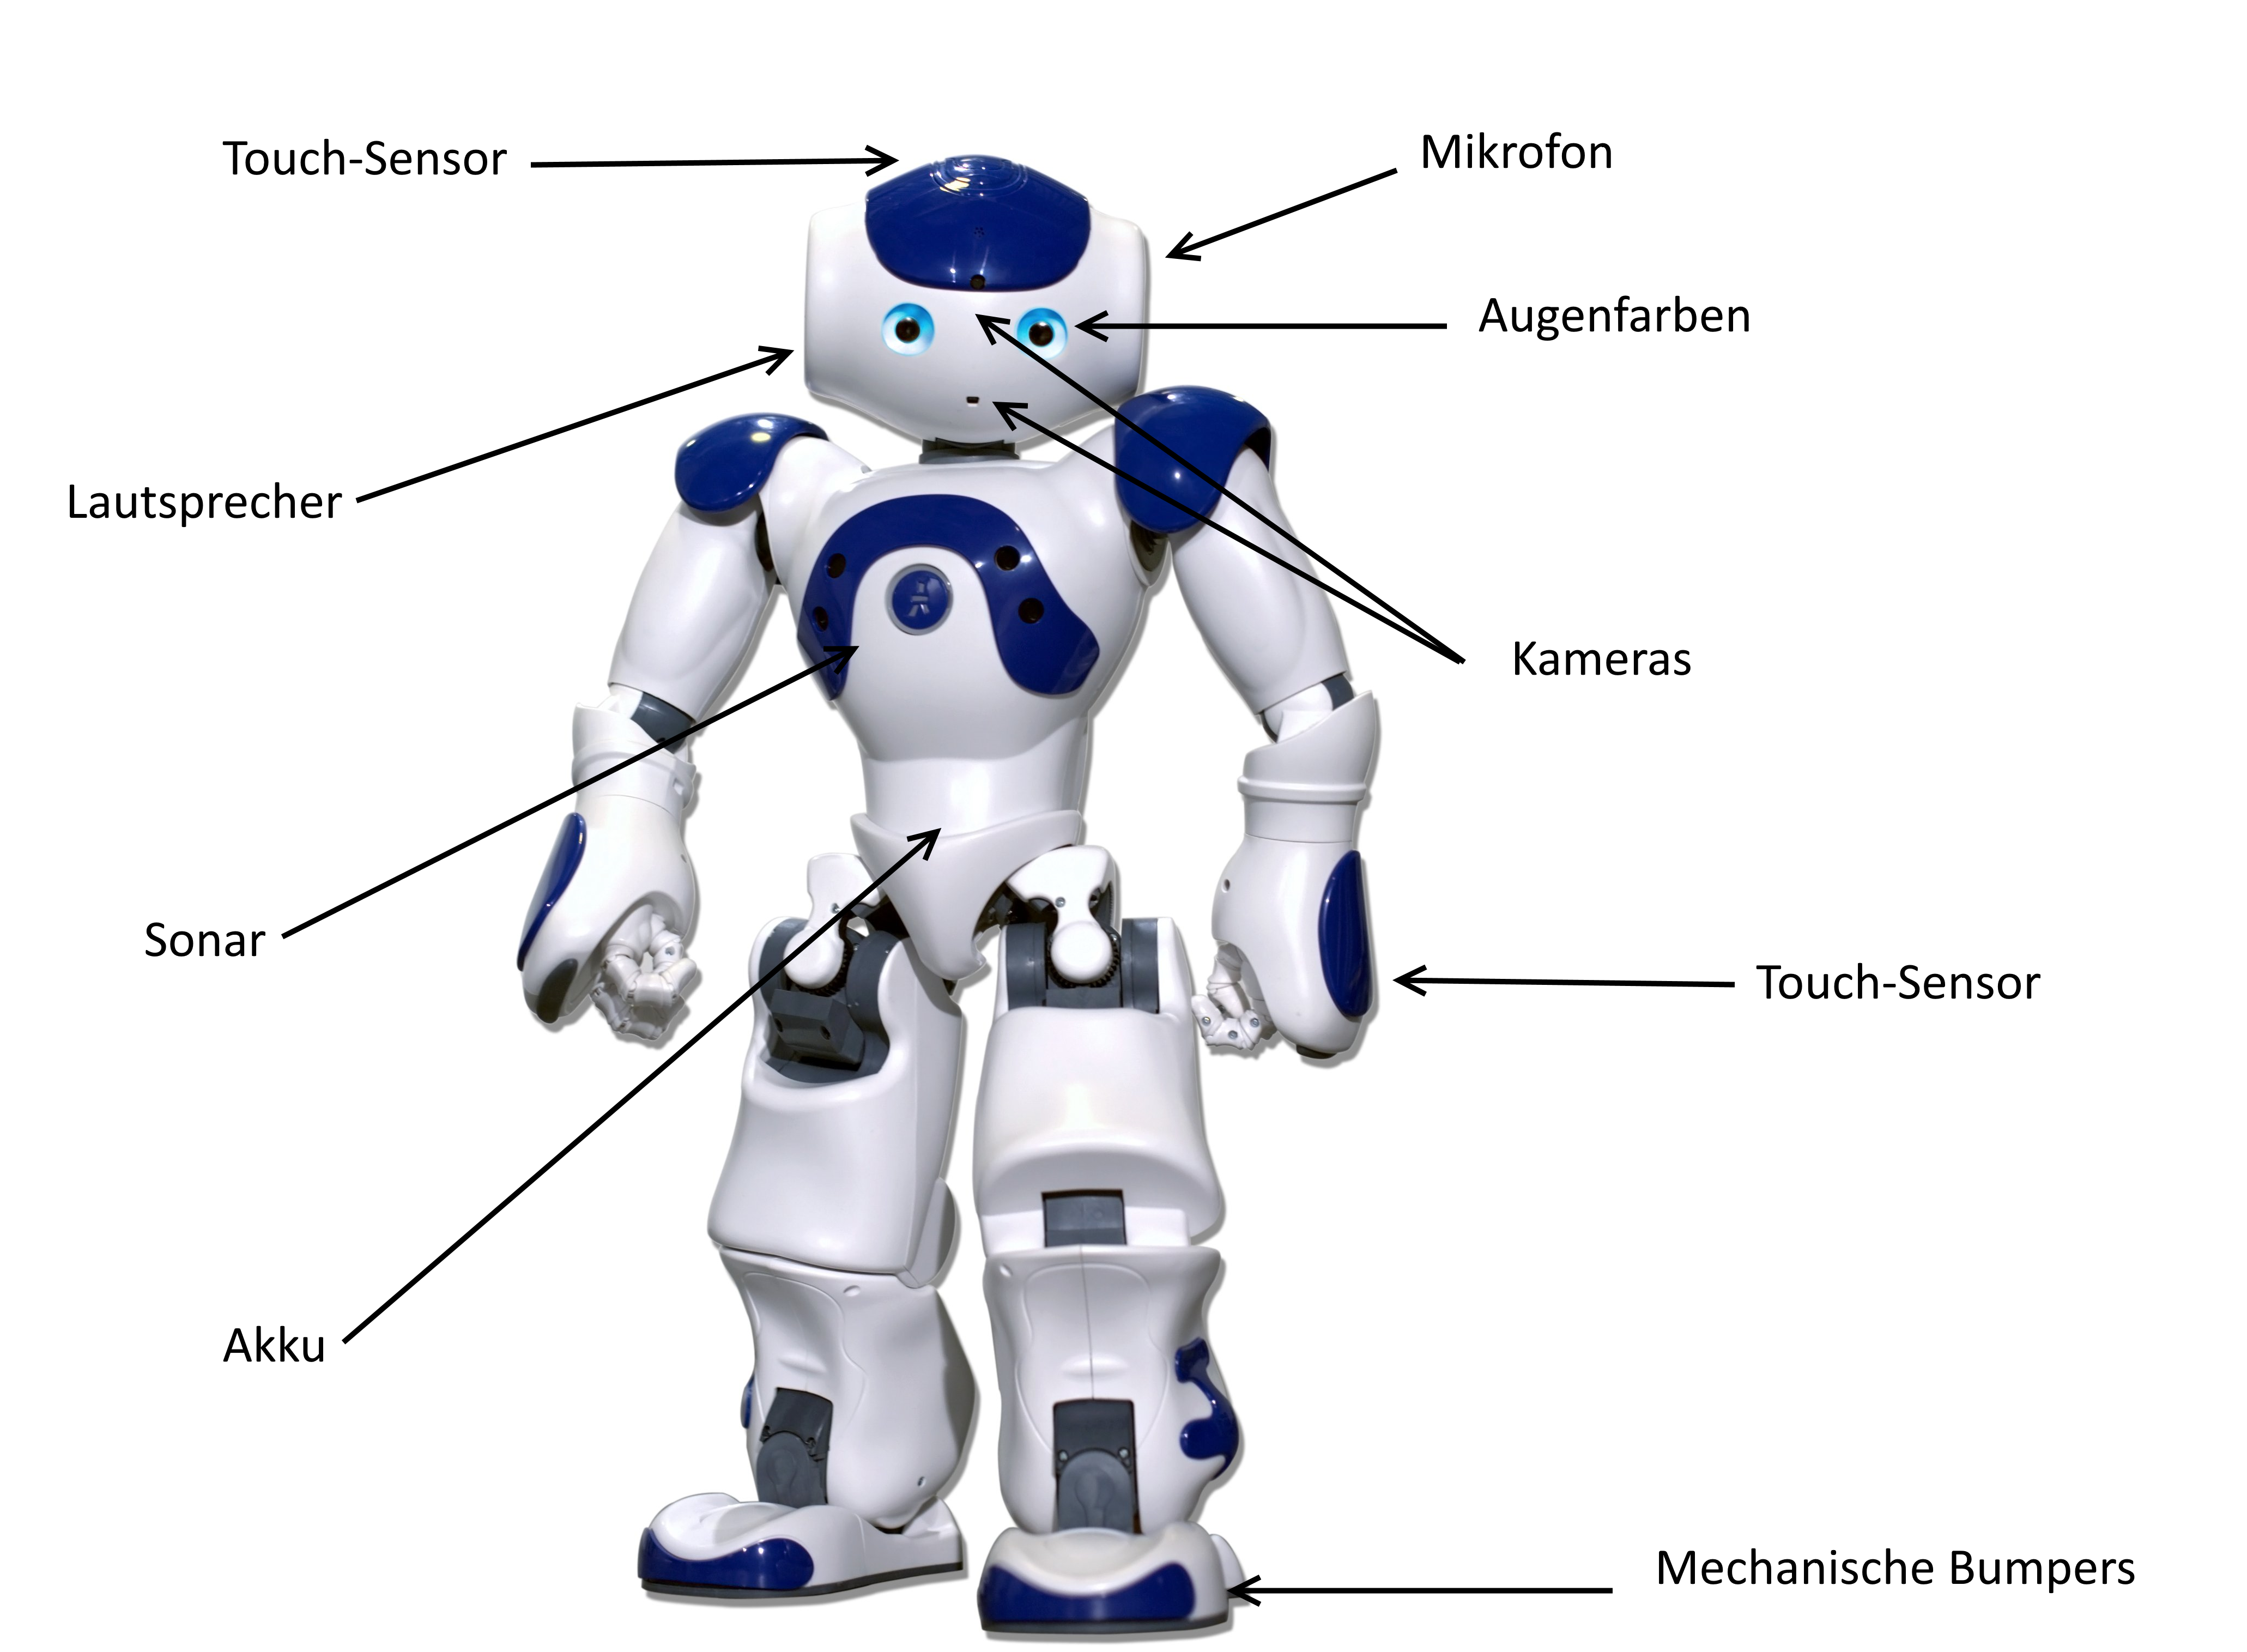
\includegraphics[width=0.99\textwidth]{src/pictures/nao-sensors.png}
            \caption{Sensoren des NAO}
            \label{img:nao:sensors}
        \end{figure}

        \begin{figure}[ht]
            \centering
            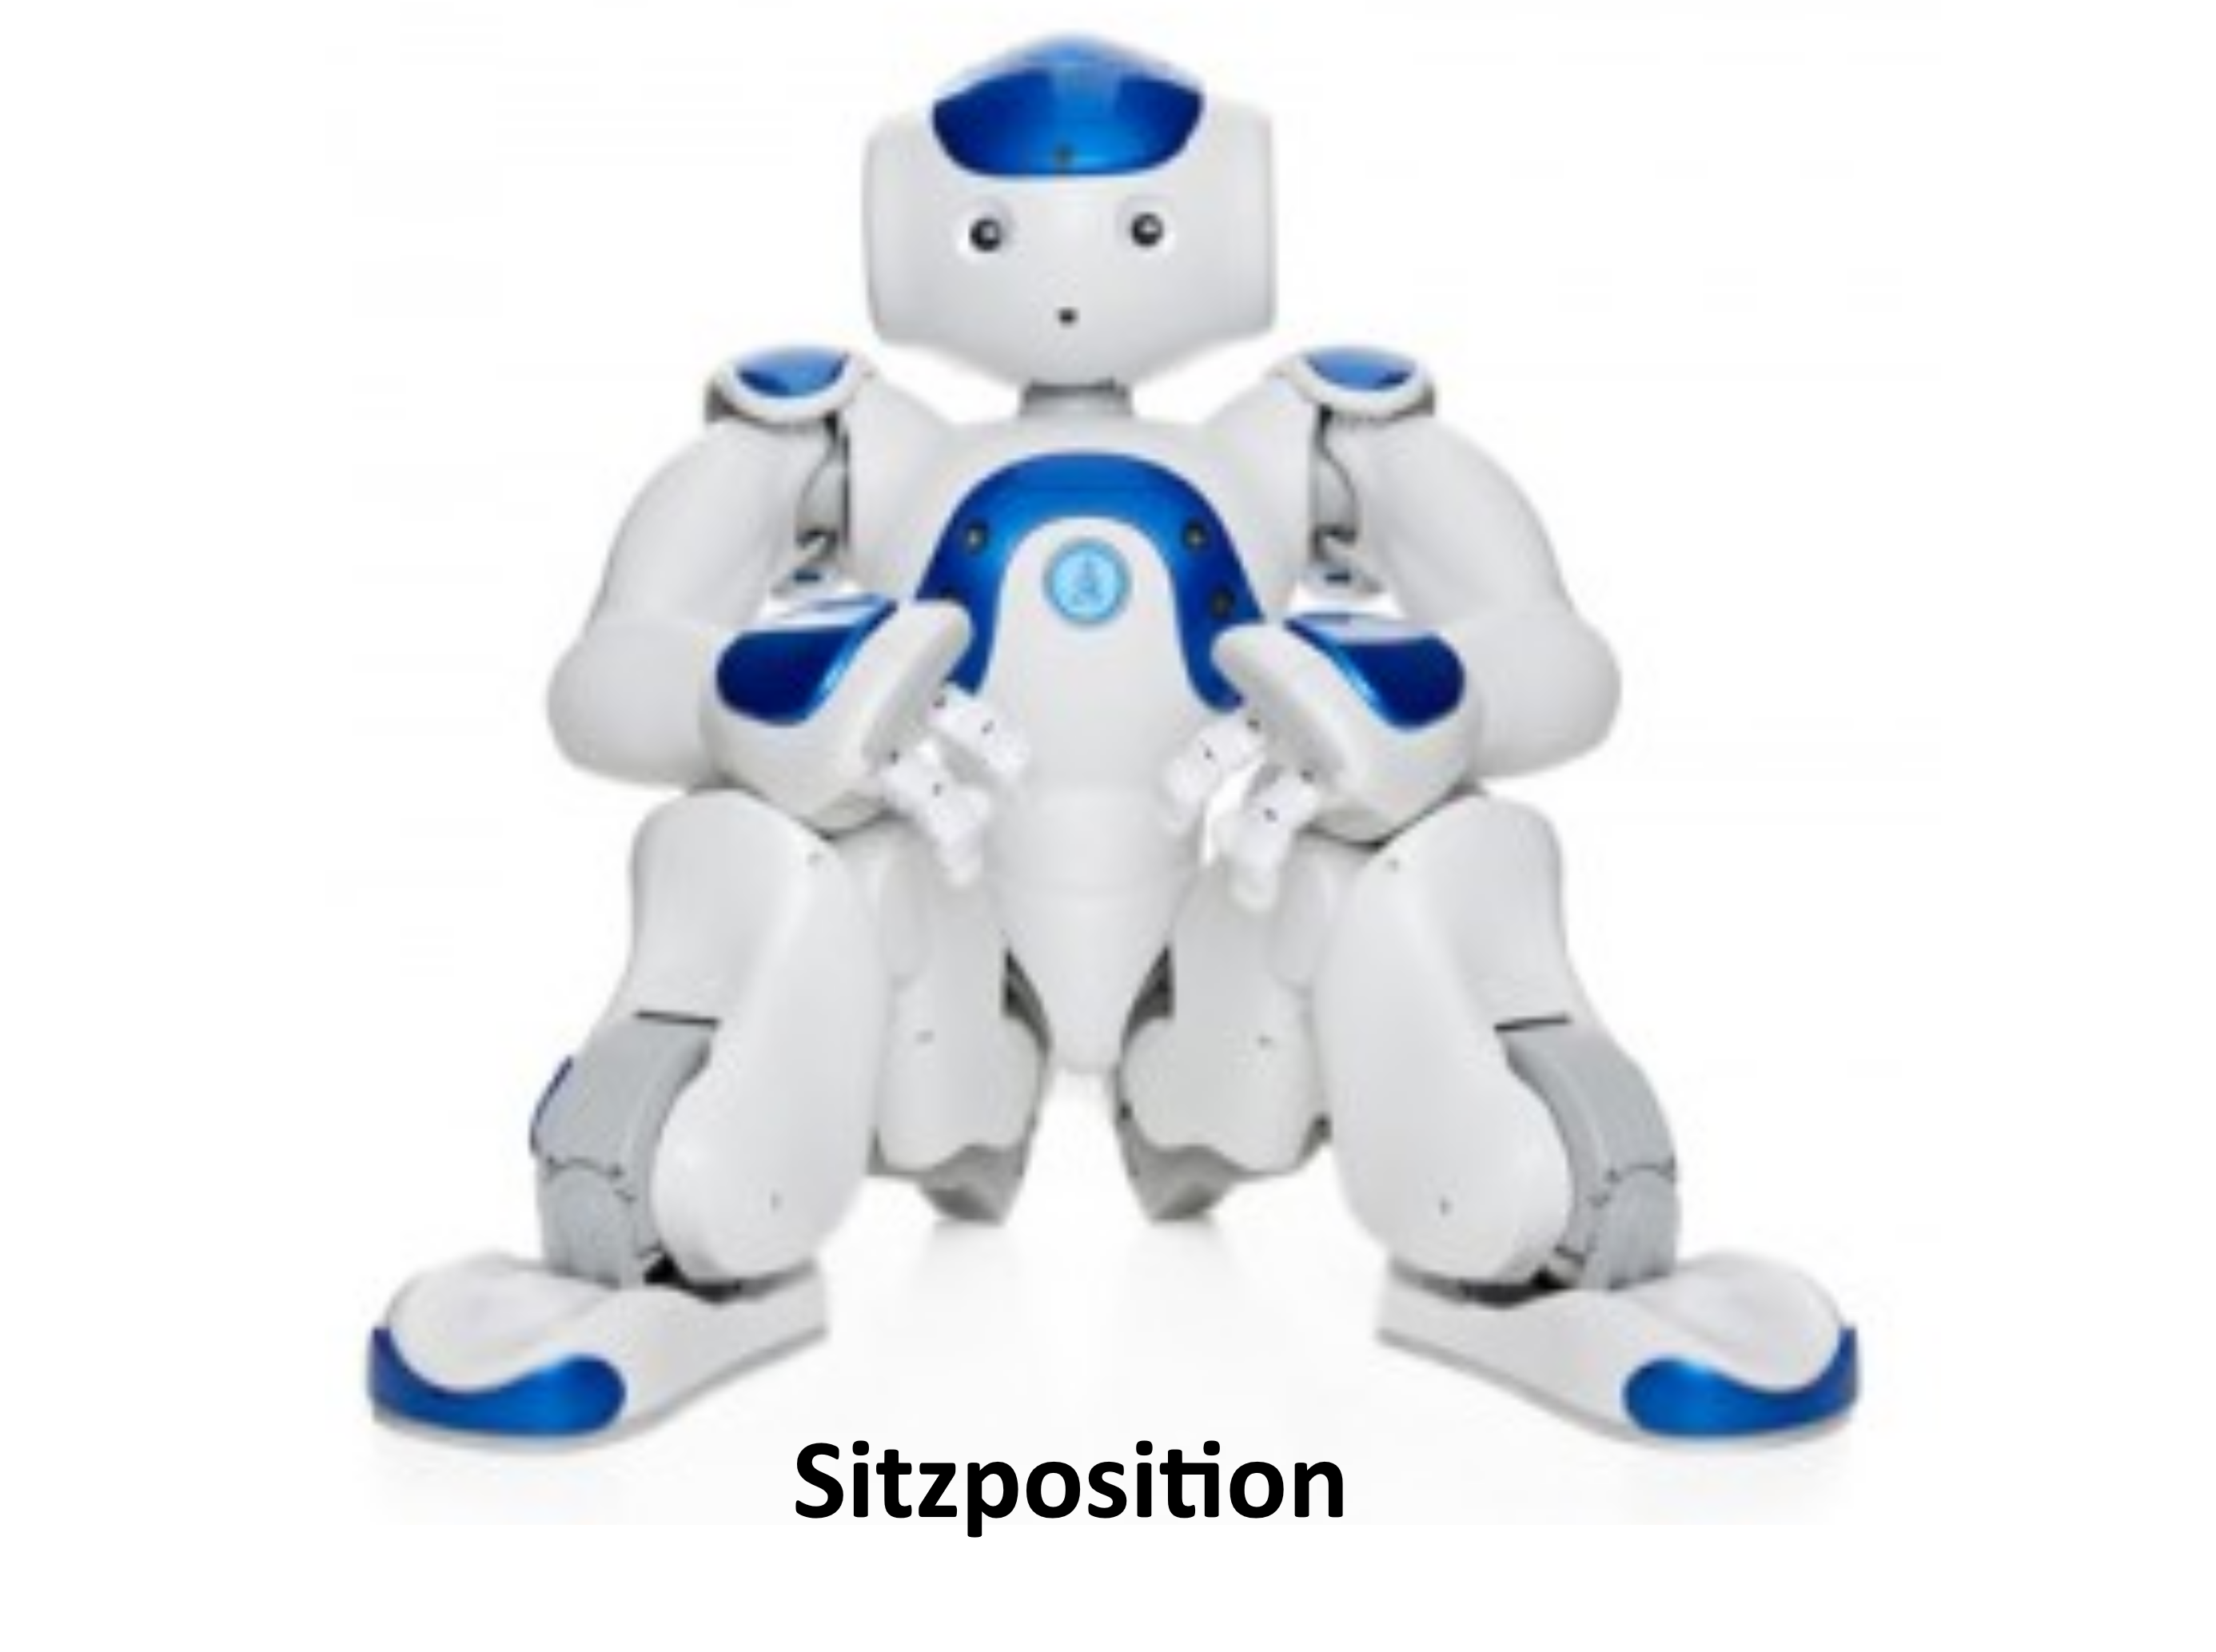
\includegraphics[width=0.99\textwidth]{src/pictures/nao-sitting.png}
            \caption{Sitzposition des NAO}
            \label{img:nao:sitting}
        \end{figure}

        \begin{figure}[ht]
            \centering
            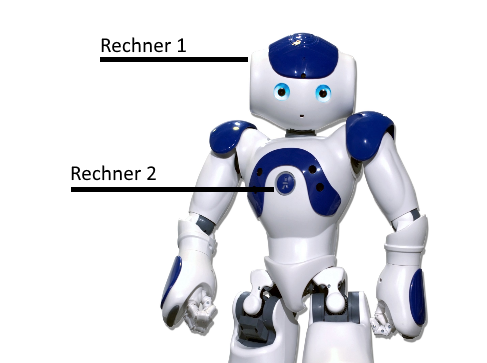
\includegraphics[width=0.99\textwidth]{src/pictures/nao-computers.png}
            \caption{Recheneinheiten des NAO}
            \label{img:nao:computers}
        \end{figure}

        \begin{figure}[ht]
            \centering
            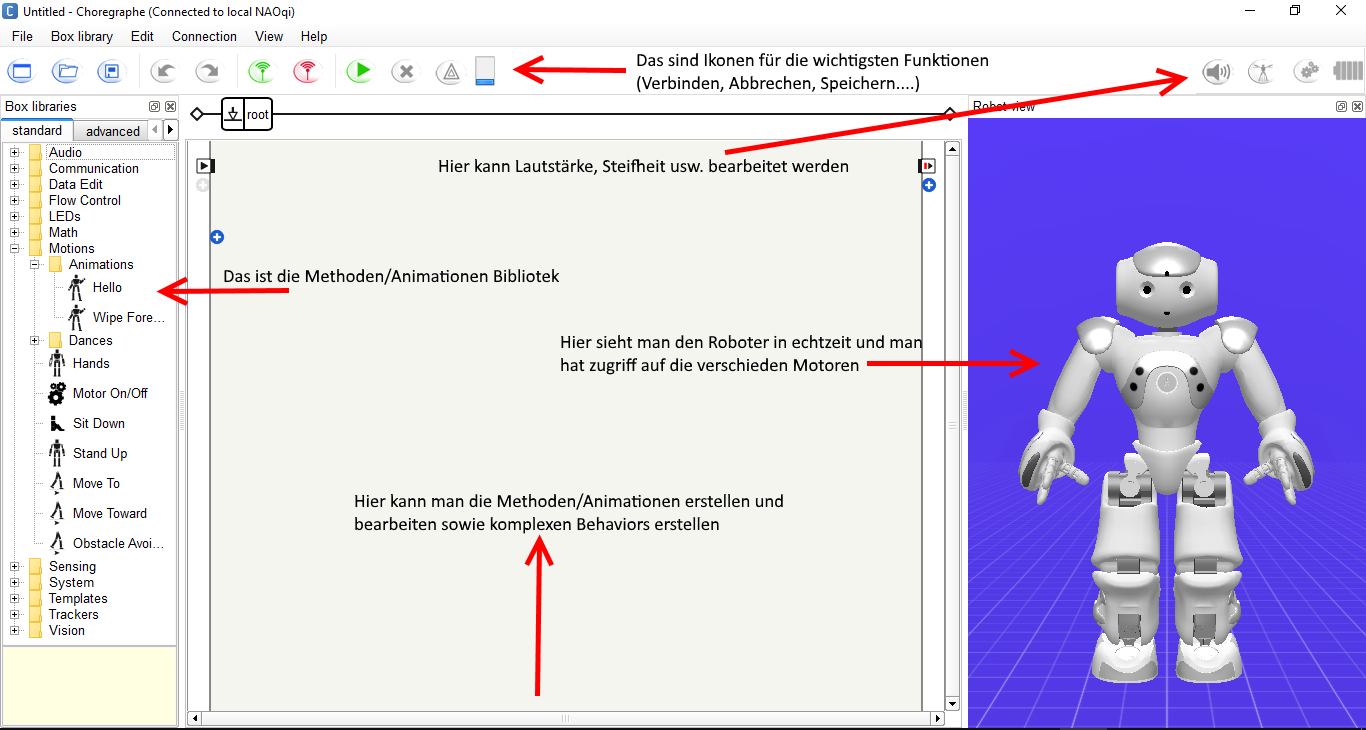
\includegraphics[angle=90, width=0.80\textwidth]{src/pictures/nao-choreo-welcome.png}
            \caption{Choreographe}
            \label{img:nao:choreo:welcome}
        \end{figure}

        \begin{figure}[ht]
            \centering
            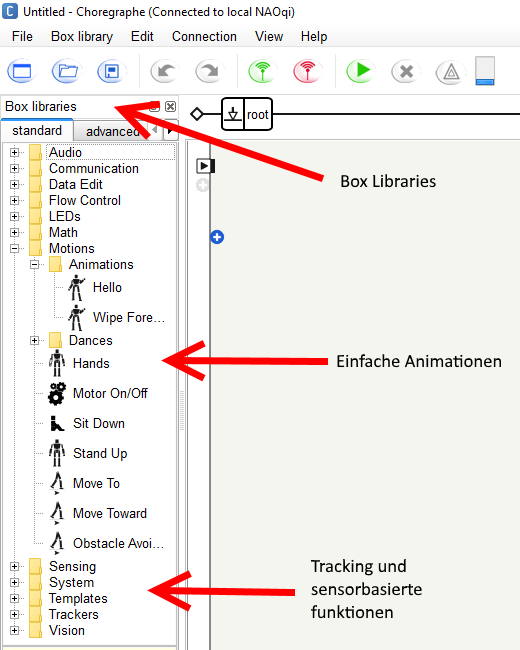
\includegraphics[width=0.99\textwidth]{src/pictures/nao-choreo-boxlib.png}
            \caption{Choreographe: Box Libraries}
            \label{img:nao:choreo:boxlib}
        \end{figure}

        \begin{figure}[ht]
            \centering
            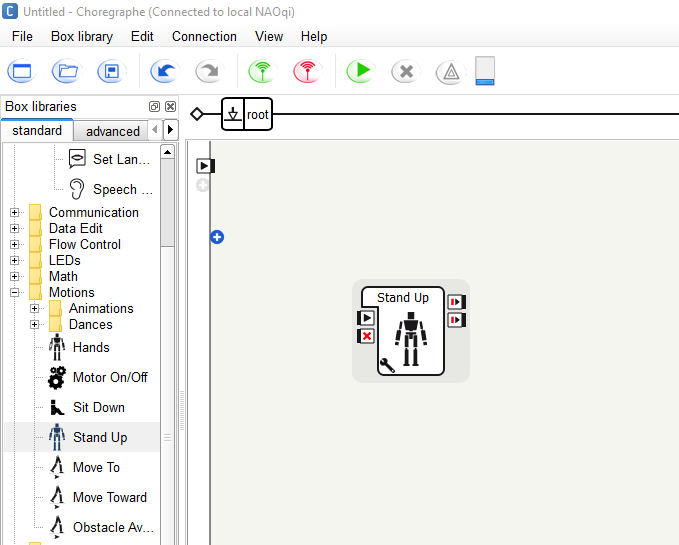
\includegraphics[width=0.99\textwidth]{src/pictures/nao-choreo-dad.png}
            \caption{Choreographe: Behaviour auf Arbeitsfläche}
            \label{img:nao:choreo:draganddrop}
        \end{figure}

        \begin{figure}[ht]
            \centering
            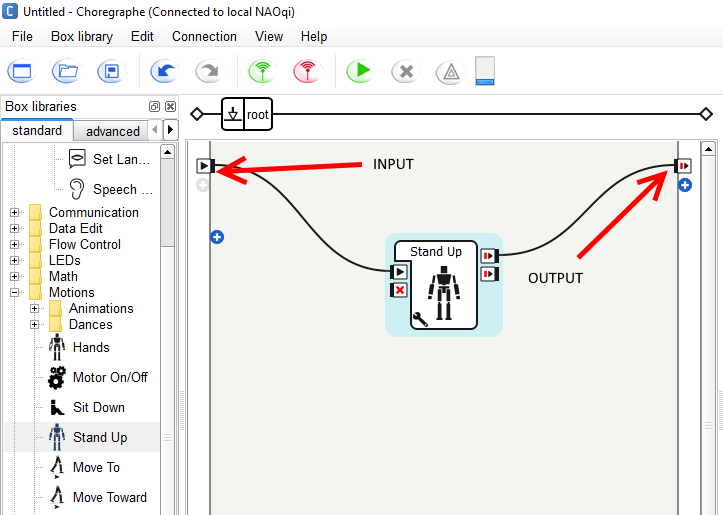
\includegraphics[width=0.99\textwidth]{src/pictures/nao-choreo-connect.png}
            \caption{Choreographe: Behaviour verbinden}
            \label{img:nao:choreo:connect}
        \end{figure}

        \begin{figure}[ht]
            \centering
            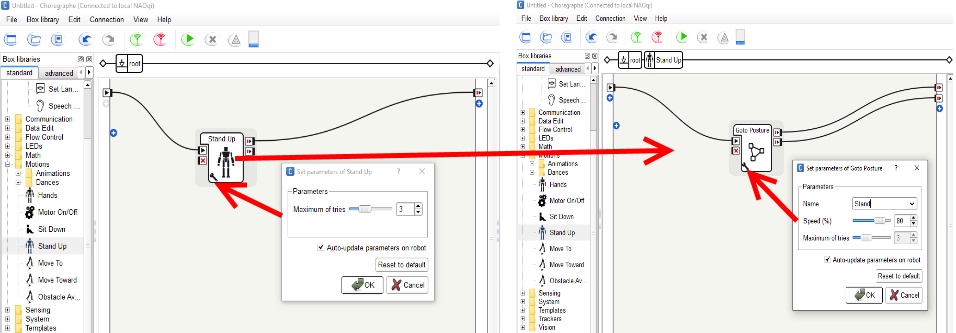
\includegraphics[width=0.99\textwidth]{src/pictures/nao-choreo-options.png}
            \caption{Choreographe: Behaviour bearbeiten}
            \label{img:nao:choreo:options}
        \end{figure}

        \cleardoubleemptypage

        \begin{figure}[ht]
            \centering
            \includegraphics[width=0.99\textwidth]{src/pictures/Packages-uml.png}
            \caption{Packages}
            \label{img:packages}
        \end{figure}

        \begin{figure}[ht]
            \centering
            \includegraphics[width=0.99\textwidth]{src/pictures/Package_Behaviour-uml.png}
            \caption{Package: Behaviour}
            \label{img:package:behaviour}
        \end{figure}

        \begin{figure}[ht]
            \centering
            \includegraphics[width=0.99\textwidth]{src/pictures/Package_OpenCV-uml.png}
            \caption{Package: OpenCV}
            \label{img:package:ocv}
        \end{figure}

        \cleardoubleemptypage

        \begin{figure}[ht]
            \centering
            \includegraphics[width=0.99\textwidth]{src/pictures/algo/usecase.png}
            \caption{Algorithmus: Usecases}
            \label{img:algo:usecases}
        \end{figure}

        \cleardoubleemptypage

        \begin{figure}[ht]
            \centering
            \includegraphics[width=0.99\textwidth]{src/pictures/Package_Algo-uml.png}
            \caption{Algorithmus: Classes}
            \label{img:algo:classes}
        \end{figure}

        \cleardoubleemptypage

        \begin{figure}[ht]
            \centering
            \includegraphics[width=0.99\textwidth]{src/pictures/algo/sequence.png}
            \caption{Algorithmus: Sequenz}
            \label{img:algo:sequence}
        \end{figure}

        \cleardoubleemptypage

        \section{Projektplan}

            \begin{figure}[ht]
                \centering
                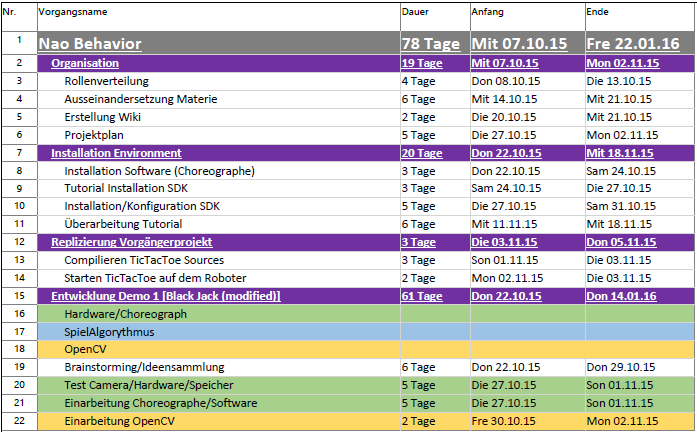
\includegraphics[width=0.99\textwidth]{src/pictures/planung1.png}
                \caption{Projektplan, Teil 1}
                \label{img:planung1}
            \end{figure}

            \begin{figure}[ht]
                \centering
                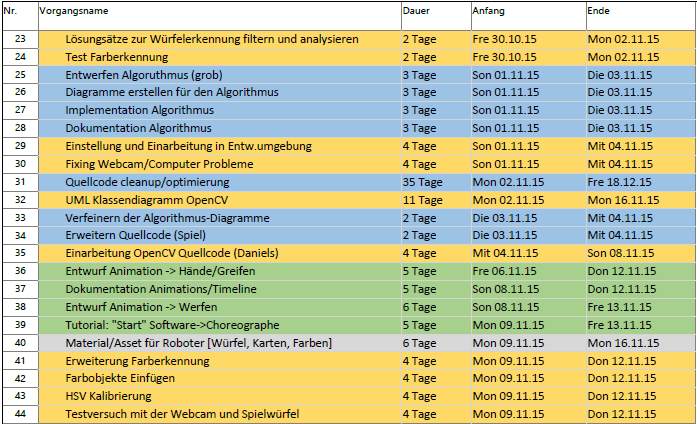
\includegraphics[width=0.99\textwidth]{src/pictures/planung2.png}
                \caption{Projektplan, Teil 2}
                \label{img:planung2}
            \end{figure}

            \begin{figure}[ht]
                \centering
                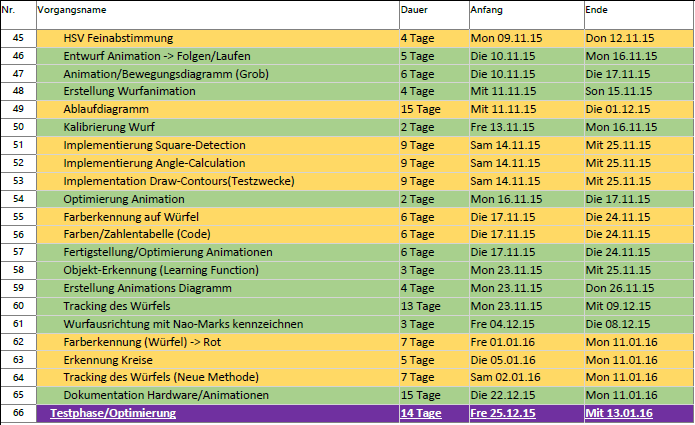
\includegraphics[width=0.99\textwidth]{src/pictures/planung3.png}
                \caption{Projektplan, Teil 3}
                \label{img:planung3}
            \end{figure}

            \begin{figure}[ht]
                \centering
                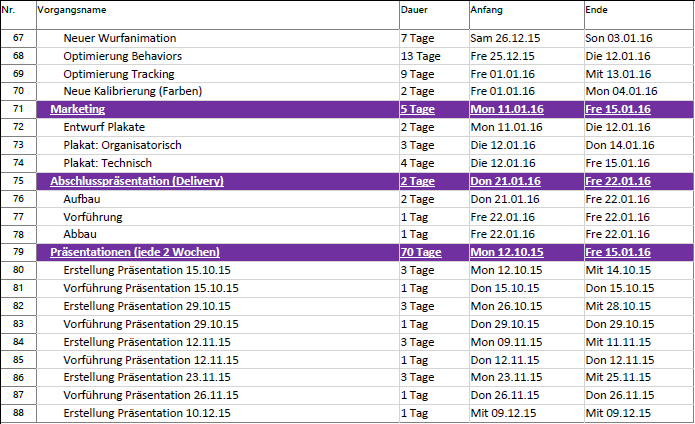
\includegraphics[width=0.99\textwidth]{src/pictures/planung4.png}
                \caption{Projektplan, Teil 4}
                \label{img:planung4}
            \end{figure}

            \begin{figure}[ht]
                \centering
                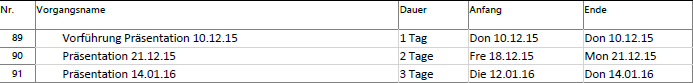
\includegraphics[width=0.99\textwidth]{src/pictures/planung5.png}
                \caption{Projektplan, Teil 5}
                \label{img:planung5}
            \end{figure}

    \chapter{Tabellen}

        \begin{table}[h]
            \caption{Koordinaten}
            \label{tbl:cmtbl}
            \begin{center}
                \begin{tabular}[]{| l | l | l |}
                    Vorgang & Verantwortlich & Dauer (Tage) \\
                    \hline

                    Einarbeitung                       &      & 14 \\
                    \hline
                    Rollenverteilung                   & Alle & 1 \\
                    Auseinandersetzung mit der Materie & Alle & 3 \\
                    Erstellung Wiki, Umgebung          & Alle & 2 \\

                    \hline

                    Replizierung Vorgängerprojekt     &                   & 14 \\
                    \hline
                    Tutorial Installation SDK         & Daniel Eisenreich & 10 \\
                    Installation Software             & Alle              & 2 \\
                    Installation/Konfiguration OpenCV & Alle              & 2 \\
                    Installation/Konfiguration SDK    & Alle              & 2 \\

                    \hline

                    Entwicklung                 &                               & \\
                    \hline
                    Brainstorming/Ideensammlung & Alle                          & 2 \\
                    Projektplan                 & Sardor Tarik, Butrint Veselaj & 10 \\
                    Klassendiagram              & Butrint Veselaj               & 1 \\
                    Modulplan                   & Butrint Veselaj               & 1 \\
                    Ablaufdiagram               & Butrint Veselaj               & 1 \\

                    \hline

                    Präsentationen            &                             & \\
                    \hline
                    Erstellung Präsentation 1 & Sardor Tarik, Matthias Kotz & 2 \\
                    Vorführung Präsentation 1 & Matthias Kotz               & 2 \\
                    Erstellung Präsentation 2 & Sardor Tarik, Matthias Kotz & 2 \\
                \end{tabular}
            \end{center}
        \end{table}[h]

        \begin{table}[h]
            \caption{Koordinaten}
            \label{tbl:cmtbl}
            \begin{center}
                \begin{tabular}[]{| l | l | l | l | l | l |}
                    \hline
                    cm      & Delta (cm) & Pixel & Differenz (px) & Quotient     & Segment \\

                    \hline

                    20      &            & 960   &                &              & \multirow{2}{1cm}{1} \\
                            & 10         &       & 208            & $20.8 px/cm$ & \\
                    \hline

                    30      &            & 752   &                &              & \multirow{2}{1cm}{2} \\
                            & 10         &       & 137            & $13.7 px/cm$ & \\
                    \hline

                    40      &            & 615   &                &              & \multirow{2}{1cm}{3} \\
                            & 10         &       & 103            & $10.3 px/cm$ & \\
                    \hline

                    50      &            & 512   &                &              & \multirow{2}{1cm}{4} \\
                            & 10         &       & 96             & $9.6 px/cm$  & \\
                    \hline

                    60      &            & 416   &                &              & \multirow{2}{1cm}{5} \\
                            & 10         &       & 71             & $7.1 px/cm$  & \\
                    \hline

                    70      &            & 345   &                &              & \multirow{2}{1cm}{6} \\
                            & 10         &       & 60             & $6.0 px/cm$  & \\
                    \hline

                    80      &            & 285   &                &              & \multirow{2}{1cm}{7} \\
                            & 10         &       & 53             & $5.3 px/cm$  & \\
                    \hline

                    90      &            & 232   &                &              & \multirow{2}{1cm}{8} \\
                            & 10         &       & 43             & $4.3 px/cm$  & \\
                    \hline

                    100     &            & 182   &                &              & \multirow{2}{1cm}{9} \\
                            & 10         &       & 39             & $3.9 px/cm$  & \\
                    \hline

                    110     &            & 150   &                &              & \multirow{3}{1cm}{10} \\
                            & 10         &       & 33             & $3.3 px/cm$  & \\
                    \hline
                    120     &            & 117   &                &              & \\
                    \hline

                \end{tabular}
            \end{center}
        \end{table}

    \chapter{Quellcode}

\begin{lstlisting}[language=c++,
                   caption={Funktion: "`getXY''},
                   label={lst:getxy}]
void getXY(float& x, float& y) {
    int start = 20; // in cm
    if(centerPoint.y >= 752) {
        x = start + (centerPoint.y - 752) / 20.8;
    }else if(centerPoint.y >= 615) {
        x = start + 10 + (centerPoint.y - 615) / 13.7;
    }else if(centerPoint.y >= 512) {
        x = start + 20 + (centerPoint.y - 512) / 10.3;
    }else if(centerPoint.y >= 416) {
        x = start + 30 + (centerPoint.y - 416) / 9.6;
    }else if(centerPoint.y >= 345) {
        x = start + 40 + (centerPoint.y - 345) / 7.1;
    }else if(centerPoint.y >= 285) {
        x = start + 50 + (centerPoint.y - 285) / 6;
    }else if(centerPoint.y >= 232) {
        x = start + 60 + (centerPoint.y - 232) / 5.3;
    }else if(centerPoint.y >= 189) {
        x = start + 70 + (centerPoint.y - 189) / 4.3;
    }else if(centerPoint.y >= 150) {
        x = start + 80 + (centerPoint.y - 150) / 3.9;
    }else if(centerPoint.y >= 117) {
        x = start + 90 + (centerPoint.y - 117) / 3.3;
    }
    y = (640 - centerPoint.x) / 14;
}
\end{lstlisting}

\begin{lstlisting}[language=c++,
                   caption={Funktion: "`getDiceValue''},
                   label={lst:getDiveValue1}]
void getDiveValue() {
    int counter = 1;
    int diffx, diffy;
    std::vector<std::shared_ptr<FarbPos>> closerSelection;

    for(int i = 0; i < farblist.size(); i++){
        if(farblist.at(i)->size > 85){
            closerSelection.push_back(farblist.at(i));
        }
    }

        counter = closerSelection.size();
    for(int i = 0; i < closerSelection.size() - 1; i++){
        for(int i2 = i + 1; i2 < closerSelection.size(); i2++){
            diffx = std::abs(closerSelection.at(i)->xPos - closerSelection.at(i2)->xPos);
            diffy = std::abs(closerSelection.at(i)->yPos - closerSelection.at(i2)->yPos);


            std::cout << "DIFF x: " << diffx << " y: " << diffy << std::endl;
            if(diffx <= 40 && diffy <= 40){
                counter--;
                break;
            }
        }
    }
    return counter;
}
\end{lstlisting}

\begin{lstlisting}[language=c++,
                   caption={Behaviour Map},
                   label={lst:behmap}]
void Behavior::initializeMap(){
    #define insert_in_map(k,v) do {                                     \
            BIDstring.insert(std::pair<BehaviorID, std::string>(k,v));  \
        } while(0)

    insert_in_map(Stand_up, "Black_Standup");
    insert_in_map(Pickup, "Black_Pickup");
    insert_in_map(Throw, "Black_Throw");
    insert_in_map(Search_Position, "Black_Search_Position");
    insert_in_map(Register_Color, "Black_Register_Color");
    insert_in_map(Search_Position, "Black_Search_Position");
    insert_in_map(Won, "Black_Won");
    insert_in_map(Lost, "Black_Lost");
    insert_in_map(Turn_Around, "Turn_Around");
    insert_in_map(Greetings, "Black_Greetings");
    insert_in_map(ALL, "");

    #undef insert_in_map
}
\end{lstlisting}

\begin{lstlisting}[language=c++,
                   caption={Behaviour Enumerator},
                   label={lst:behstart}]
void Behavior::startBehavior(BehaviorID BID){
    switch(BID) {
        case 0:
            std::cout << "STANDUP" << std::endl;
            globalBehaveProxy->runBehavior(BIDstring[Stand_up]);
            break;
        case 1:
            globalBehaveProxy->runBehavior(BIDstring[Pickup]);
            break;
        case 2:
            globalBehaveProxy->runBehavior(BIDstring[Throw]);
            break;
        case 3:
            globalBehaveProxy->runBehavior(BIDstring[Register_Color]);
            break;
        case 4:
            globalBehaveProxy->runBehavior(BIDstring[Search_Position]);
            break;
        case 5:
            globalBehaveProxy->runBehavior(BIDstring[Won]);
            break;
        case 6:
            globalBehaveProxy->runBehavior(BIDstring[Lost]);
            break;
        case 8:
            globalBehaveProxy->runBehavior(BIDstring[Greetings]);
            break;
    }
}
\end{lstlisting}

\begin{lstlisting}[language=c++,
                   caption={Behaviour Enumerator},
                   label={lst:behstop}]

void Behavior::stopBehavior(BehaviorID BID){
    switch(BID) {
        case 0:
            globalBehaveProxy->stopBehavior(BIDstring[Stand_up]);
            break;
        case 1:
            globalBehaveProxy->stopBehavior(BIDstring[Pickup]);
            break;
        case 2:
            globalBehaveProxy->stopBehavior(BIDstring[Throw]);
            break;
        case 3:
            globalBehaveProxy->stopBehavior(BIDstring[Register_Color]);
            break;
        case 4:
            globalBehaveProxy->stopBehavior(BIDstring[Search_Position]);
            break;
        case 5:
            globalBehaveProxy->stopBehavior(BIDstring[Won]);
            break;
        case 6:
            globalBehaveProxy->stopBehavior(BIDstring[Lost]);
            break;
        case 7:
            globalBehaveProxy->stopBehavior(BIDstring[Turn_Around]);
            break;
        case 8:
            globalBehaveProxy->stopBehavior(BIDstring[Greetings]);
        case 9:
            globalBehaveProxy->stopAllBehaviors();
            break;
    }
}
\end{lstlisting}

\begin{lstlisting}[language=c++,
                   caption={Mainloop},
                   label={lst:main1}]
do {
    behaviorProxy.startBehavior(behavior::Pickup);
    int g; std::cin >> g;
    BehaviorProxy.startBehavior(behavior::Throw);
    behaviorProxy.startBehavior(behavior::Stand_up);
    behaviorProxy.startBehavior(behavior::Search_Position);
    speakProxy.say("Ich suche jetzt den Wuerfel");
    imageLoaderProxy.getImage();

    for(int i = 0; naocv::colorDetection(pathToFile, x, y, angle) == 0; i++){
        if(i == 0){
            navigationProxy.moveTo(0, 0, 0.95);
            behaviorProxy.startBehavior(behavior::Search_Position);
            imageLoaderProxy.getImage();
        }
        else if(i == 1){
            navigationProxy.moveTo(0, 0, -1.7472);
            behaviorProxy.startBehavior(behavior::Search_Position);
            imageLoaderProxy.getImage();
        }
        else if(i == 2){
            navigationProxy.moveTo(0, 0, 0.95);
            navigationProxy.moveTo(-0.2, 0, 0);
            behaviorProxy.startBehavior(behavior::Search_Position);
            imageLoaderProxy.getImage();
            if(naocv::colorDetection(pathToFile, x, y, angle) != 0){
                cubeFound = true;
            }
        }
        else {
            if(cubeFound)
                break;
            else{
                speakProxy.say("Ich habe den Wuerfel nicht gefunden!");
                throw std::runtime_error("Cube not Found");
            }
        }
    }

    speakProxy.say("Ich habe den Wuerfel gefunden");

    x = x * 0.01; // cm in m
    y = y * 0.01; // cm in m
    y = y + -(x * 0.005); //compensate slip
    angle = (-(x * 0.00581776) * 0.2);
    navigationProxy.moveTo(0, y, 0);
    navigationProxy.moveTo(x / 2, 0, angle);

    navigationProxy.moveTo(x, 0, angle);

    speakProxy.say("Nun schaue ich welche Zahl ich habe");
    behaviorProxy.startBehavior(behavior::Register_Color);
    imageLoaderProxy.getImage();
    auto analyzed = naocv::colorDetection(pathToFile, x, y, angle, false);

    algo.update(std::make_shared<algo::Card>(analyzed));
    draw = algo.doDraw();

    speakProxy.say("Ich habe eine");
    speakProxy.say(naocv::intTostring(analyzed));

    if (counter > 0) {
        speakProxy.say(",Insgesamt habe ich");
        speakProxy.say(naocv::intTostring(algo.get_current_sum()));
    }

    if (draw) {
        speakProxy.say("Ich wuerfel noch ein mal");
    }

    counter++;
} while (draw);

int state = algo.getState();
std::cout << "SUM: " << algo.get_current_sum() << std::endl;
std::cout << "STATE: " << state << std::endl;
speakProxy.say("ich bin fertig mit wuerfeln");

if (state == 4) {
    speakProxy.say("Glueckwunsch, du hast gewonnen!");
    behaviorProxy.startBehavior(behavior::Lost);
} else if (state == 3) {
    if (algo.get_current_sum() == 21) {
        behaviorProxy.startBehavior(behavior::Won);
    } else {
        speakProxy.say("Jetzt darfst du wuerfeln!");
        int z;
        std::cin >> z;
        speakProxy.say("Nun schaue ich welche Zahl du gewuerfelt hast");
        behaviorProxy.startBehavior(behavior::Register_Color);
        imageLoaderProxy.getImage();
        auto analyzed = naocv::colorDetection(pathToFile, x, y, angle, false);
        speakProxy.say("Du hast eine");
        speakProxy.say(naocv::intTostring(analyzed));
        int newSum = algo.get_current_sum() + analyzed;
        if (newSum <= 21) {
            speakProxy.say("Glueckwunsch, du hast gewonnen!");
            behaviorProxy.startBehavior(behavior::Lost);
        } else {
            behaviorProxy.startBehavior(behavior::Won);
        }
\end{lstlisting}

\end{appendix}
